\documentclass[xcolor=dvipsnames,t]{beamer} 

\usepackage{listings} 
\usepackage{color} 
\usepackage{xcolor}  
\usepackage{microtype} 
\usepackage{helvet} 
\usepackage{inconsolata} 
\usepackage[framemethod=TikZ]{mdframed} 
\usepackage{graphicx} 
\usepackage{alltt}
\usepackage{sverb} 
\usepackage{verbatim} 
\usepackage{pifont} 
\usepackage{alltt} 
\usepackage{helvet} 

\usetheme{Madrid} 

\setbeamertemplate{navigation symbols}{}
\setbeamertemplate{blocks}[default] 

%\definecolor{mypurple}{rgb}{.49,0,98}
%\setbeamercolor*{palette primary}{use=structure,fg=white,bg=green}
%\usecolortheme[rgb={0.9,0.2,0.2}]{structure}
%\usecolortheme[rgb={0.6,0.1,0.1}]{structure}
\usecolortheme[rgb={0.4, 0.0, 0.4}]{structure} 

\usepackage{color}
\definecolor{orange}{cmyk}{0,0.4,0.8,0.2}
\definecolor{darkorange}{rgb}{.71,0.21,0.01}
\definecolor{darkgreen}{rgb}{.12,.54,.11}
\definecolor{myteal}{rgb}{.26, .44, .56}
\definecolor{gray}{gray}{0.45}
\definecolor{lightgray}{gray}{.95}
\definecolor{mediumgray}{gray}{.8}
\definecolor{inputbackground}{rgb}{.95, .95, .85}
\definecolor{outputbackground}{rgb}{.95, .95, .95}
\definecolor{traceback}{rgb}{1, .95, .95}
\definecolor{inputbg}{rgb}{0.98, 0.98, 0.98}

\usepackage{listings} 
\lstset{language=c,
        %basicstyle=\footnotesize\ttfamily, 
        basicstyle=\small\ttfamily,
        columns=fullflexible, 
        %title=\lstname, 
        %numbers=left, stringstyle=\texttt, 
        %numberstyle={\tiny\texttt}, 
        keywordstyle=\color{blue}, 
        commentstyle=\color{darkgreen}, 
        stringstyle=\color{purple} } 


\mdfsetup{skipabove=\topskip, skipbelow=\topskip} 

\definecolor{codebg}{rgb}{0.99,0.99,0.99}

\global\mdfdefinestyle{code}{%
    frametitlerule=true,%
    frametitlefont=\small\bfseries\ttfamily,%
    frametitlebackgroundcolor=lightgray,%
    backgroundcolor=codebg,%
    linecolor=gray, linewidth=0.5pt,%
    leftmargin=0.5cm, rightmargin=0.5cm,%
    roundcorner=2pt,%
    innerleftmargin=5pt
}

\global\mdfdefinestyle{code2}{%
    topline=false,%
    bottomline=false,%
    leftline=true,%
    rightline=false,%
    backgroundcolor=codebg,%
    linecolor=gray, linewidth=0.5pt,%
    leftmargin=0.0cm, rightmargin=0.0cm,%
    innerleftmargin=1pt
}

\newcommand{\showcode}[1]{\begin{mdframed}[style=code] %
                            \lstinputlisting{#1}% 
                          \end{mdframed}% 
}


\title[OpenGL]{Introduction to OpenGL}
\subtitle{Graphics and Computation} 
\author{Michael Papasimeon} % \\
\date{2005, 2006, 2007} 

\begin{document}

\begin{frame}
    \maketitle
\end{frame} 

\begin{frame}{Outline}
    \begin{itemize}
        \item OpenGL Background and History
        \item Other Graphics Technologies
        \item Drawing
        \item Viewing and Transformation
        \item Lighting
        \item GLUT and JOGL
        \item Resources
    \end{itemize} 
\end{frame}

\begin{frame}{OpenGL Background and History} 
    \begin{itemize}
        \item OpenGL = Open Graphics Library
        \item Developed at Silicon Graphics (SGI)
        \item Successor to IrisGL
        \item Cross Platform (Win32, Mac OS X, Unix, Linux)
        \item Only does 3D Graphics. No Platform Specifics (Windowing, Fonts, Input, GUI)
        \item Version 1.4 widely available
        \item Two Libraries
        \begin{itemize}
            \item GL (Graphics Library)
            \item GLU (Graphics Library Utilities)
        \end{itemize} 
    \end{itemize} 
\end{frame} 

\begin{frame}{Other Graphics Technologies} 
    \begin{itemize}
        \item Low level graphics
        \item OpenGL
        \item Scene Graphs, BSPs
            \begin{itemize}
                \item OpenSceneGraph, Java3D, VRML, PLIB
            \end{itemize} 
        \item DirectX - Direct3D
        \item Can mix some DirectX with OpenGL (e.g. in Quake III OpenGL is used w/ DirectInput)
    \end{itemize} 
\end{frame} 

\begin{frame}{Platform Specifics}
    \begin{itemize}
        \item Platform Specific OpenGL Interfaces
            \begin{itemize} 
                \item Windows - WGL
                \item XWindows X11 - GLX
                \item Mac OS X - CGL/AGL/NSOpenGL
                \item Motif - GLwMwidget
                \item Qt - QGLWidget, QGLContext
            \end{itemize} 
        \item GLUT - GL Utility Library (C, Python, ...)
        \item JOGL (Java)
    \end{itemize} 
\end{frame} 

\begin{frame}{The Drawing Process}
    \showcode{draw.c} 
    \begin{itemize} 
        \item In animation there are usually two buffers. 
        \item Drawing usually occurs on the background buffer. 
        \item When it is complete, it is brought to the front (swapped). 
        \item This gives a smooth animation without the viewer seeing the 
              actual drawing taking place. 
        \item Only the final image is viewed.
        \item The technique to swap the buffers will depend on which 
              windowing library you are using with OpenGL.
    \end{itemize} 
\end{frame} 

\begin{frame}{Clearing the Window} 
    \showcode{clearcolor.c} 
    Typically you would clear the colour and depth buffers together.
    \showcode{clear.c} 
\end{frame} 

\begin{frame}{Setting the Colour} 
    \begin{itemize}
        \item Colour is specified in (R,G,B,A) form [Red, Green, Blue, Alpha].
        \item Each value being in the range of $0.0$ to $1.0$.
        \item There are many variants of the glColor command.
    \end{itemize} 
    \begin{block}{Specifying Colour with \texttt{glColor}}
        \showcode{color.c} 
    \end{block} 
\end{frame} 

\begin{frame}{Complete Drawing the Scene} 
    Need to tell OpenGL you have finished drawing your scene:
    \showcode{glfinish.c} 
    or
    \showcode{glflush.c} 
    For more information see:\\
    \small
    \url{http://www.rush3d.com/reference/opengl-redbook-1.1/chapter02.html}
    \normalsize
\end{frame} 

\begin{frame}{Drawing in OpenGL}
    \begin{itemize} 
        \item Use \texttt{glBegin()} to start drawing and \texttt{glEnd()} to stop.
        \item \texttt{glBegin()} can draw in many different styles.
        \item \texttt{glVertex3f(x,y,z)} specifies a point in 3D space.
    \end{itemize} 
    \begin{block}{Drawing a Polygon} 
        \showcode{polygon.c} 
    \end{block} 
\end{frame} 

\begin{frame}{\texttt{glBegin} Drawing Modes}  
    \begin{center} 
         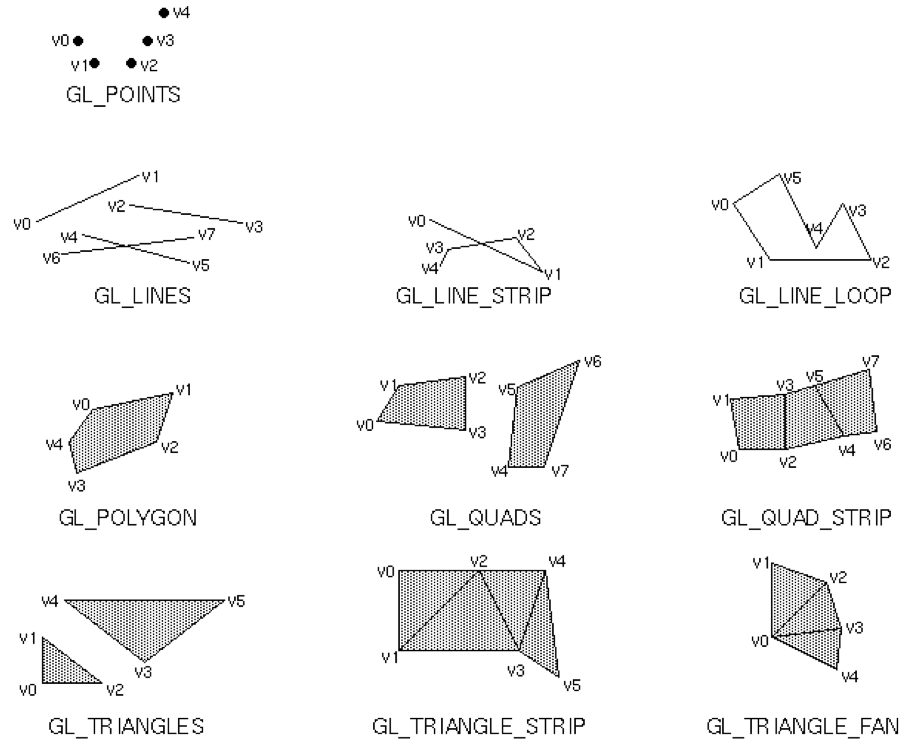
\includegraphics[width=0.7\textwidth]{glbegin} 
    \end{center} 
\end{frame} 

\begin{frame}{Mixing Geometry with Colour} 
    Specifying vertices can be mixed with colour and other 
    types of commands for interesting drawing results.
    \showcode{geomcolor.c} 
\end{frame} 

\begin{frame}{Viewing the Scene: The Camera}
\end{frame} 

\begin{frame}{OpenGL Vertices} 
    \begin{itemize}
        \item OpenGL uses a 4-component vector to represent a vertex.
        \item Known as homogenous coordinate system~\footnote{For 
            further information on homogenous coordinate systems as 
            used in projective geometry and in OpenGL, see Appendix G of the Red Book
            \url{http://www.rush3d.com/reference/opengl-redbook-1.1/appendixg.html} } 
            where typically $w=1$.
        \item In 2D-space $z=0$.
    \end{itemize} 
    \begin{equation*}
        v = \left( 
                \begin{array}{c}
                x \\
                y \\
                z \\
                w
                \end{array}
            \right)
    \end{equation*} 
\end{frame} 

\begin{frame}{Vertex Transformations} 
\end{frame} 

\begin{frame}{Vertex Transformation as Matrix Multiplication} 
    \begin{equation*}
        v' = M v
    \end{equation*} 
    \vspace{1cm} 
    \begin{equation*} 
        M = \left(
                \begin{array}{cccc}
                    m_{1}   & m_{5}     & m_{9}     & m_{13} \\
                    m_{2}   & m_{6}     & m_{10}    & m_{14} \\
                    m_{3}   & m_{7}     & m_{11}    & m_{15} \\
                    m_{4}   & m_{8}     & m_{12}    & m_{16} 
                \end{array} 
            \right)
    \end{equation*} 
\end{frame} 

\begin{frame}{The ModelView Matrix}
    \texttt{glMatrixMode(GL\_MODELVIEW);} \\[1cm]
    Specifying the \texttt{ModelView} matrix is analogous to:
    \begin{itemize} 
        \item Positioning and aiming the camera (viewing transformation)
        \item Positioning and orienting the model (modeling transformation)
    \end{itemize} 
\end{frame} 

\begin{frame}{The Projection Matrix}
\texttt{glMatrixMode(GL\_PROJECTION);} \\[1cm]
    \begin{itemize} 
        \item Specifiying the \texttt{Projection} matrix is like chosing a lens for a camera.
        \item It lets you specify parameters such as the field of view.
    \end{itemize} 
\end{frame} 

\begin{frame}{OpenGL Matrix Operations} 
    Identity Matrix
    \begin{equation*}
    I = \left(
                \begin{array}{cccc}
                    1   & 0     & 0     & 0     \\
                    0   & 1     & 0     & 0     \\
                    0   & 0     & 1     & 0     \\
                    0   & 0     & 0     & 1
                \end{array} 
            \right)
    \end{equation*} 
    \showcode{matrixops.c} 
\end{frame} 

\begin{frame}{Perspective Projection (glFrustrum)}
\end{frame} 

\begin{frame}{Perspective Projection (gluPerspective) from GLU} 
\end{frame} 

\begin{frame}{Orthographics (Parallel) Projection - glOrtho} 
\end{frame} 

\begin{frame}{gluLookAt}
\end{frame} 

\begin{frame}{Translation Transformation}
\end{frame} 

\begin{frame}{Rotation Transformations} 
\end{frame} 

\begin{frame}{Scaling Transformations} 
\end{frame} 

\begin{frame}{Order of Transformations}
\end{frame} 

\begin{frame}{Transformations in Action}
\end{frame} 

\begin{frame}{The Matrix Stack} 
\end{frame} 

\begin{frame}{OpenGL Lighting} 
\end{frame} 

\begin{frame}{Setting up an OpenGL Light}
    \showcode{light.c} 
\end{frame} 

\begin{frame}{glLight\{if\}[v](light, pname, param)}
\end{frame} 

\begin{frame}{Material Properties} 
\end{frame} 

\begin{frame}{glMaterial Default Parameters} 
\end{frame} 

\begin{frame}{Teapots Materials Example} 
\end{frame} 

\begin{frame}{Normal Vectors} 
\end{frame} 

\begin{frame}{Normal Vectors (2)}
\end{frame} 

\begin{frame}{Hidden Surface Removal} 
\end{frame} 

\begin{frame}{GLUT} 
\end{frame} 

\begin{frame}{Example GLUT Program in C} 
    \showcode{glutmain.c} 
\end{frame} 

\begin{frame}{Typical InitGL() Function} 
    \showcode{initgl.c} 
\end{frame} 

\begin{frame}{Typical GLUT Reshape Function} 
    \showcode{reshape.c} 
\end{frame} 

\begin{frame}{Typical GLUT Display Function} 
    \showcode{display.c} 
\end{frame} 

\begin{frame}{JOGL} 
\end{frame} 

\begin{frame}{JOGL Example} 
\end{frame} 

\begin{frame}{JOpenGLDemoClass}
\end{frame} 

\begin{frame}{JOGL Main Method} 
\end{frame} 

\begin{frame}{JOGL Init Method} 
\end{frame} 

\begin{frame}{JOGL Reshape (Window Resize) Method} 
\end{frame}

\begin{frame}{JOGL Display Method} 
\end{frame} 

\begin{frame}{JOGL Demo} 
\end{frame} 

\begin{frame}{JOGL on Mac OS X} 
\end{frame} 

\begin{frame}{OpenGL Books} 
\end{frame} 

\begin{frame}{Resources} 
\end{frame} 

\begin{frame}{Project Preparation} 
\end{frame} 

\end{document}
